\documentclass[a4paper,11pt,dvipdfmx]{ujarticle}
% パッケージ
\usepackage{graphicx}
\usepackage{url}
% レイアウト指定を記述したファイルの読み込み
\input{layout}

% タイトルと氏名を変更せよ.
\title{日本におけるデジタルの状況}
\author{G584092025 - ZEYAR MIN ZIN}

\begin{document}

\maketitle

\section{ブロードバンドの整備状況}

OCEDによるブロードバンド回線の普及の関する調査\cite{oecd}によると,図\ref{fig:いち}に示すように, 日本における100人あたりのモバイルブロードバンドの加入者数は190.5で, 第1位になっている, 2位はエストニアで, 3位米国と続く.

\begin{figure}[htbp]
    \centering
    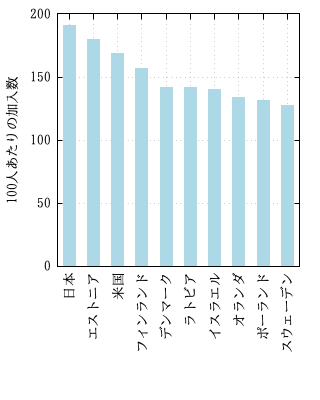
\includegraphics[scale=0.8]{fig21.png}
    \caption{光ファイバー回線の加入者数(100人あたり)}\label{fig:いち}
\end{figure}

\newpage
\section{デジタル競争力ランキング}

国際経営開発研究所(IMD)の調査\cite{imd}によると、表\ref{tbl:に}に示すように、日本のデジタル競争力のランキングは調査対象の64カ国中、総合で28位、知識分野で25位となっている。

\begin{table}[htbp]
    \centering
    \caption{:デジタル競争力ランキング(64カ国中)}\label{tbl:に}
    \begin{tabular}{|c|c|c|}\hline
        国 & 総合 & 知識 \\
        \hline
        米国 & 1位 & 3位\\
        \hline
        香港 & 2位 & 5位\\
        \hline
        スウェーデン & 3位 & 2位\\
        \hline
        デンマーク & 4位 & 8位\\
        \hline
        シンガポール & 5位 & 4位\\
        \hline
        \hline
        韓国 & 12位 & 15位\\
        \hline 
        中国 & 15位 & 6位\\
        \hline
        \hline
        日本 & 28位 & 25位 \\
        \hline
    \end{tabular}
\end{table}

\section{考察}
\begin{itemize}
    \item 日本はインターネットの環境はいいです。
    \item デジタルの力はまだ弱いです。
    \item 人と会社がもっとデジタルを使うことが大事です
\end{itemize}



\bibliographystyle{junsrt}
\bibliography{exercise.bib}

\end{document}